\documentclass[12pt]{article}
\usepackage{graphicx}
\begin{document}
\title{Computer Science M151B, Homework 1}
\date{April 9th, 2018}
\author{Michael Wu\\UID: 404751542}
\maketitle

\section*{Problem 1}

\begin{figure}[ht]
    \begin{center}
        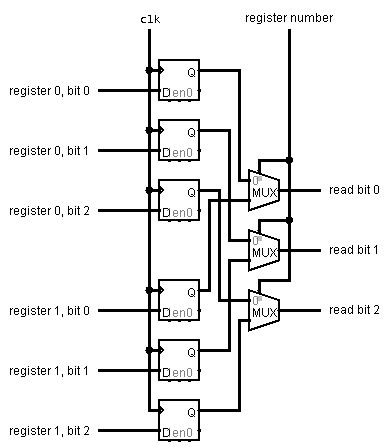
\includegraphics[width=3.5in]{problem1.png}
    \end{center}
\end{figure}

\section*{Problem 2}

\begin{verbatim}
addi $9,  $5,  -12
add  $10, $5,  $8
sll  $9,  $9,  2
sll  $10, $10, 2
lui  $11, 0x351C
slr  $11, $11, 16
lui  $11, 0x3B
add  $9,  $9,  $11
add  $10, $10, $11
lw   $12, 0($10)
sub  $12, $12, $13
sw   $12, 0($9)
\end{verbatim}

\section*{Problem 3}

\begin{verbatim}
addi $8,  $0,  0xFF
sll  $8,  $8,  10
and  $9,  $14, $8
sll  $9,  $9,  14
sll  $8,  $8,  14
nor  $8,  $8,  $0
and  $22, $22, $8
or   $22, $22, $9
\end{verbatim}

\section*{Problem 4}

\begin{verbatim}
slt  $20, $0,  $17 # $0 < $17, so $20=1
bne  $20, $0,  1   # $20 != $0, so increase program counter by 1
beq  $0,  $0,  1   # skipped
addi $20, $20, 2   # $20 = $20 + 2, so $20=3
\end{verbatim}
The final value of register \texttt{\$20} is \(3\). The flow of execution is such that the first instruction stores \(1\) in register
\texttt{\$20}, which then causes the next instruction to branch. This skips the third instruction, and finally the last instruction adds
\(2\) to register \texttt{\$20} and stores it, resulting in the value of \(3\).

\section*{Problem 5}

The machine code in binary is
\begin{verbatim}
1001 0110 1100 1110 0000 0000 0010 1101
\end{verbatim}

\section*{Problem 6}

\begin{center}
        \hspace*{-1cm}
        \begin{tabular}{|c||c|c|c|c|c|c|c|}
                \hline
                Address & op & rs & rt & rd & shamt & func & inst \\
                \hline\hline
                0000 0001 1100 0100 & 001000 & 00000 & 01111 & \multicolumn{3}{|c|}{0000 0000 0010 0001} & addi\\
                \hline
                0000 0001 1100 1000 & 000000 & 00000 & 00101 & 00100 & 00010 & 000000 & sll\\
                \hline
                0000 0001 1100 1100 & 000000 & 01011 & 00100 & 00100 & 00000 & 100000& add\\
                \hline
                0000 0001 1101 0000 & 100011 & 00100 & 00100 & \multicolumn{3}{|c|}{0000 0000 0000 0000} & lw\\
                \hline
                0000 0001 1101 0100 & 000100 & 00100 & 01111 & \multicolumn{3}{|c|}{0000 0000 0000 0111} & beq\\
                \hline
                0000 0001 1101 1000 & 001000 & 00101 & 00101 & \multicolumn{3}{|c|}{0000 0000 0000 0001} & addi\\
                \hline
                0000 0001 1101 1100 & 000000 & 00111 & 00100 & 00011 & 00000 & 101010 & slt\\
                \hline
                0000 0001 1110 0000 & 000100 & 00011 & 00000 & \multicolumn{3}{|c|}{0000 0000 0000 0010} & beq\\
                \hline
                0000 0001 1110 0100 & 000000 & 01100 & 00100 & 01100 & 00000 & 100000 & add\\
                \hline
                0000 0001 1110 1000 & 000010 & \multicolumn{5}{|c|}{00 0000 0000 0000 0000 0111 0010} & j\\
                \hline
                0000 0001 1110 1100 & 000000 & 01100 & 00111 & 01100 & 00000 & 100010 & sub\\
                \hline
                0000 0001 1111 0000 & 000010 & \multicolumn{5}{|c|}{00 0000 0000 0000 0000 0111 0010} & j\\
                \hline
        \end{tabular}
        \hspace*{-1cm}
\end{center}

\section*{Problem 7}

\begin{verbatim}
sltu $13, $25, $22
\end{verbatim}
No assumptions are made, this exactly captures the functionality of \texttt{sgtu}.

\section*{Problem 8}

\begin{verbatim}
lui  $8,  0x5D2C
slr  $8,  $8,  16
lui  $8,  0x34
lw   $8,  0($8)
lui  $9,  0x9878
slr  $9,  $9,  16
lui  $9,  0xDABA
beq  $5,  $8,  1
jr   $9
\end{verbatim}
This code loads both 32-bit immediates into registers \texttt{\$8} and \texttt{\$9}, then uses a branch if equal to skip a jump instruction.
The address stored at register \texttt{\$8} is dereferenced using the load word instruction, and then compared to register \texttt{\$5}.
If register \texttt{\$5} and the value at \texttt{\$8} is equal, no jump happens due to the branch. Otherwise the values are not equal, and
a jump will happen to the address given by the second immediate, which is stored in register \texttt{\$9}. An assumption is that registers
\texttt{\$8} and \texttt{\$9} are not already being used.

\section*{Problem 9}

\begin{verbatim}
addi $4,  $0,  1
sll  $4,  $4,  24
sw   $4,  8($0)
lb   $4,  8($0)   # 0 if little endian, 1 if big endian
sb   $4,  129($0)
\end{verbatim}
This code puts the hex value \texttt{0x01000000} into register \texttt{\$4}, then stores register \texttt{\$4} into main memory at addresses
\(8\)-\(11\). Because this is done using a store word operation, the order of the bytes depend on whether the computer is little endian or big endian.
The code then loads the byte at address \(8\) to check endianness. If the computer is big endian a \(1\) should have been loaded, otherwise a
\(0\) should have been loaded. Finally the program stores the byte that was loaded into the byte at address \(129\).

\end{document}
